\documentclass[1p]{elsarticle_modified}
%\bibliographystyle{elsarticle-num}

%\usepackage[colorlinks]{hyperref}
%\usepackage{abbrmath_seonhwa} %\Abb, \Ascr, \Acal ,\Abf, \Afrak
\usepackage{amsfonts}
\usepackage{amssymb}
\usepackage{amsmath}
\usepackage{amsthm}
\usepackage{scalefnt}
\usepackage{amsbsy}
\usepackage{kotex}
\usepackage{caption}
\usepackage{subfig}
\usepackage{color}
\usepackage{graphicx}
\usepackage{xcolor} %% white, black, red, green, blue, cyan, magenta, yellow
\usepackage{float}
\usepackage{setspace}
\usepackage{hyperref}

\usepackage{tikz}
\usetikzlibrary{arrows}

\usepackage{multirow}
\usepackage{array} % fixed length table
\usepackage{hhline}

%%%%%%%%%%%%%%%%%%%%%
\makeatletter
\renewcommand*\env@matrix[1][\arraystretch]{%
	\edef\arraystretch{#1}%
	\hskip -\arraycolsep
	\let\@ifnextchar\new@ifnextchar
	\array{*\c@MaxMatrixCols c}}
\makeatother %https://tex.stackexchange.com/questions/14071/how-can-i-increase-the-line-spacing-in-a-matrix
%%%%%%%%%%%%%%%

\usepackage[normalem]{ulem}

\newcommand{\msout}[1]{\ifmmode\text{\sout{\ensuremath{#1}}}\else\sout{#1}\fi}
%SOURCE: \msout is \stkout macro in https://tex.stackexchange.com/questions/20609/strikeout-in-math-mode

\newcommand{\cancel}[1]{
	\ifmmode
	{\color{red}\msout{#1}}
	\else
	{\color{red}\sout{#1}}
	\fi
}

\newcommand{\add}[1]{
	{\color{blue}\uwave{#1}}
}

\newcommand{\replace}[2]{
	\ifmmode
	{\color{red}\msout{#1}}{\color{blue}\uwave{#2}}
	\else
	{\color{red}\sout{#1}}{\color{blue}\uwave{#2}}
	\fi
}

\newcommand{\Sol}{\mathcal{S}} %segment
\newcommand{\D}{D} %diagram
\newcommand{\A}{\mathcal{A}} %arc


%%%%%%%%%%%%%%%%%%%%%%%%%%%%%5 test

\def\sl{\operatorname{\textup{SL}}(2,\Cbb)}
\def\psl{\operatorname{\textup{PSL}}(2,\Cbb)}
\def\quan{\mkern 1mu \triangleright \mkern 1mu}

\theoremstyle{definition}
\newtheorem{thm}{Theorem}[section]
\newtheorem{prop}[thm]{Proposition}
\newtheorem{lem}[thm]{Lemma}
\newtheorem{ques}[thm]{Question}
\newtheorem{cor}[thm]{Corollary}
\newtheorem{defn}[thm]{Definition}
\newtheorem{exam}[thm]{Example}
\newtheorem{rmk}[thm]{Remark}
\newtheorem{alg}[thm]{Algorithm}

\newcommand{\I}{\sqrt{-1}}
\begin{document}

%\begin{frontmatter}
%
%\title{Boundary parabolic representations of knots up to 8 crossings}
%
%%% Group authors per affiliation:
%\author{Yunhi Cho} 
%\address{Department of Mathematics, University of Seoul, Seoul, Korea}
%\ead{yhcho@uos.ac.kr}
%
%
%\author{Seonhwa Kim} %\fnref{s_kim}}
%\address{Center for Geometry and Physics, Institute for Basic Science, Pohang, 37673, Korea}
%\ead{ryeona17@ibs.re.kr}
%
%\author{Hyuk Kim}
%\address{Department of Mathematical Sciences, Seoul National University, Seoul 08826, Korea}
%\ead{hyukkim@snu.ac.kr}
%
%\author{Seokbeom Yoon}
%\address{Department of Mathematical Sciences, Seoul National University, Seoul, 08826,  Korea}
%\ead{sbyoon15@snu.ac.kr}
%
%\begin{abstract}
%We find all boundary parabolic representation of knots up to 8 crossings.
%
%\end{abstract}
%\begin{keyword}
%    \MSC[2010] 57M25 
%\end{keyword}
%
%\end{frontmatter}

%\linenumbers
%\tableofcontents
%
\newcommand\colored[1]{\textcolor{white}{\rule[-0.35ex]{0.8em}{1.4ex}}\kern-0.8em\color{red} #1}%
%\newcommand\colored[1]{\textcolor{white}{ #1}\kern-2.17ex	\textcolor{white}{ #1}\kern-1.81ex	\textcolor{white}{ #1}\kern-2.15ex\color{red}#1	}

{\Large $\underline{12n_{0878}~(K12n_{0878})}$}

\setlength{\tabcolsep}{10pt}
\renewcommand{\arraystretch}{1.6}
\vspace{1cm}\begin{tabular}{m{100pt}>{\centering\arraybackslash}m{274pt}}
\multirow{5}{120pt}{
	\centering
	\includegraphics[width=112pt]{../../../GIT/diagram.site/Diagrams/png/2967_12n_0878.png}\\
\ \ \ A knot diagram\footnotemark}&
\allowdisplaybreaks
\textbf{Linearized knot diagam} \\
\cline{2-2}
 &
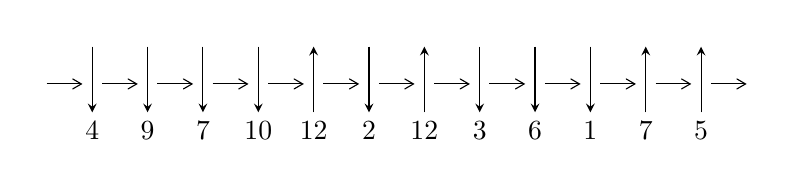
\begin{tikzpicture}[x=20pt, y=17pt]
	% nodes
	\node (C0) at (0, 0) {};
	\node (C1) at (1, 0) {};
	\node (C1U) at (1, +1) {};
	\node (C1D) at (1, -1) {4};

	\node (C2) at (2, 0) {};
	\node (C2U) at (2, +1) {};
	\node (C2D) at (2, -1) {9};

	\node (C3) at (3, 0) {};
	\node (C3U) at (3, +1) {};
	\node (C3D) at (3, -1) {7};

	\node (C4) at (4, 0) {};
	\node (C4U) at (4, +1) {};
	\node (C4D) at (4, -1) {10};

	\node (C5) at (5, 0) {};
	\node (C5U) at (5, +1) {};
	\node (C5D) at (5, -1) {12};

	\node (C6) at (6, 0) {};
	\node (C6U) at (6, +1) {};
	\node (C6D) at (6, -1) {2};

	\node (C7) at (7, 0) {};
	\node (C7U) at (7, +1) {};
	\node (C7D) at (7, -1) {12};

	\node (C8) at (8, 0) {};
	\node (C8U) at (8, +1) {};
	\node (C8D) at (8, -1) {3};

	\node (C9) at (9, 0) {};
	\node (C9U) at (9, +1) {};
	\node (C9D) at (9, -1) {6};

	\node (C10) at (10, 0) {};
	\node (C10U) at (10, +1) {};
	\node (C10D) at (10, -1) {1};

	\node (C11) at (11, 0) {};
	\node (C11U) at (11, +1) {};
	\node (C11D) at (11, -1) {7};

	\node (C12) at (12, 0) {};
	\node (C12U) at (12, +1) {};
	\node (C12D) at (12, -1) {5};
	\node (C13) at (13, 0) {};

	% arrows
	\draw[->,>={angle 60}]
	(C0) edge (C1) (C1) edge (C2) (C2) edge (C3) (C3) edge (C4) (C4) edge (C5) (C5) edge (C6) (C6) edge (C7) (C7) edge (C8) (C8) edge (C9) (C9) edge (C10) (C10) edge (C11) (C11) edge (C12) (C12) edge (C13) ;	\draw[->,>=stealth]
	(C1U) edge (C1D) (C2U) edge (C2D) (C3U) edge (C3D) (C4U) edge (C4D) (C5D) edge (C5U) (C6U) edge (C6D) (C7D) edge (C7U) (C8U) edge (C8D) (C9U) edge (C9D) (C10U) edge (C10D) (C11D) edge (C11U) (C12D) edge (C12U) ;
	\end{tikzpicture} \\
\hhline{~~} \\& 
\textbf{Solving Sequence} \\ \cline{2-2} 
 &
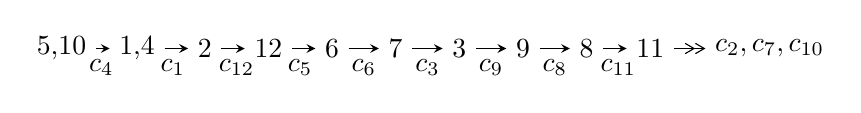
\begin{tikzpicture}[x=23pt, y=7pt]
	% node
	\node (A0) at (-1/8, 0) {5,10};
	\node (A1) at (17/16, 0) {1,4};
	\node (A2) at (17/8, 0) {2};
	\node (A3) at (25/8, 0) {12};
	\node (A4) at (33/8, 0) {6};
	\node (A5) at (41/8, 0) {7};
	\node (A6) at (49/8, 0) {3};
	\node (A7) at (57/8, 0) {9};
	\node (A8) at (65/8, 0) {8};
	\node (A9) at (73/8, 0) {11};
	\node (C1) at (1/2, -1) {$c_{4}$};
	\node (C2) at (13/8, -1) {$c_{1}$};
	\node (C3) at (21/8, -1) {$c_{12}$};
	\node (C4) at (29/8, -1) {$c_{5}$};
	\node (C5) at (37/8, -1) {$c_{6}$};
	\node (C6) at (45/8, -1) {$c_{3}$};
	\node (C7) at (53/8, -1) {$c_{9}$};
	\node (C8) at (61/8, -1) {$c_{8}$};
	\node (C9) at (69/8, -1) {$c_{11}$};
	\node (A10) at (11, 0) {$c_{2},c_{7},c_{10}$};

	% edge
	\draw[->,>=stealth]	
	(A0) edge (A1) (A1) edge (A2) (A2) edge (A3) (A3) edge (A4) (A4) edge (A5) (A5) edge (A6) (A6) edge (A7) (A7) edge (A8) (A8) edge (A9) ;
	\draw[->>,>={angle 60}]	
	(A9) edge (A10);
\end{tikzpicture} \\ 

\end{tabular} \\

\footnotetext{
The image of knot diagram is generated by the software ``\textbf{Draw programme}" developed by Andrew Bartholomew(\url{http://www.layer8.co.uk/maths/draw/index.htm\#Running-draw}), where we modified some parts for our purpose(\url{https://github.com/CATsTAILs/LinksPainter}).
}\phantom \\ \newline 
\centering \textbf{Ideals for irreducible components\footnotemark of $X_{\text{par}}$} 
 
\begin{align*}
I^u_{1}&=\langle 
1.21141\times10^{651} u^{110}-1.08774\times10^{651} u^{109}+\cdots+1.65962\times10^{652} b-7.59921\times10^{651},\\
\phantom{I^u_{1}}&\phantom{= \langle  }-1.93122\times10^{651} u^{110}+2.08824\times10^{651} u^{109}+\cdots+1.65962\times10^{652} a+1.24469\times10^{652},\\
\phantom{I^u_{1}}&\phantom{= \langle  }u^{111}- u^{110}+\cdots-7 u+3\rangle \\
I^u_{2}&=\langle 
1.42494\times10^{88} u^{41}-3.45989\times10^{87} u^{40}+\cdots+6.00691\times10^{88} b+5.71024\times10^{88},\\
\phantom{I^u_{2}}&\phantom{= \langle  }3.70120\times10^{88} u^{41}-6.96687\times10^{87} u^{40}+\cdots+6.00691\times10^{88} a+1.88942\times10^{89},\;u^{42}+7 u^{40}+\cdots+4 u+1\rangle \\
\\
\end{align*}
\raggedright * 2 irreducible components of $\dim_{\mathbb{C}}=0$, with total 153 representations.\\
\footnotetext{All coefficients of polynomials are rational numbers. But the coefficients are sometimes approximated in decimal forms when there is not enough margin.}
\newpage
\renewcommand{\arraystretch}{1}
\centering \section*{I. $I^u_{1}= \langle 1.21\times10^{651} u^{110}-1.09\times10^{651} u^{109}+\cdots+1.66\times10^{652} b-7.60\times10^{651},\;-1.93\times10^{651} u^{110}+2.09\times10^{651} u^{109}+\cdots+1.66\times10^{652} a+1.24\times10^{652},\;u^{111}- u^{110}+\cdots-7 u+3 \rangle$}
\flushleft \textbf{(i) Arc colorings}\\
\begin{tabular}{m{7pt} m{180pt} m{7pt} m{180pt} }
\flushright $a_{5}=$&$\begin{pmatrix}1\\0\end{pmatrix}$ \\
\flushright $a_{10}=$&$\begin{pmatrix}0\\u\end{pmatrix}$ \\
\flushright $a_{1}=$&$\begin{pmatrix}0.116365 u^{110}-0.125826 u^{109}+\cdots+7.34809 u-0.749986\\-0.0729930 u^{110}+0.0655417 u^{109}+\cdots-3.44083 u+0.457888\end{pmatrix}$ \\
\flushright $a_{4}=$&$\begin{pmatrix}1\\- u^2\end{pmatrix}$ \\
\flushright $a_{2}=$&$\begin{pmatrix}0.164158 u^{110}-0.170164 u^{109}+\cdots+11.2042 u-1.23626\\-0.0749935 u^{110}+0.0663564 u^{109}+\cdots-3.32164 u+0.468253\end{pmatrix}$ \\
\flushright $a_{12}=$&$\begin{pmatrix}0.189358 u^{110}-0.191368 u^{109}+\cdots+10.7889 u-1.20787\\-0.0729930 u^{110}+0.0655417 u^{109}+\cdots-3.44083 u+0.457888\end{pmatrix}$ \\
\flushright $a_{6}=$&$\begin{pmatrix}0.196495 u^{110}-0.170592 u^{109}+\cdots+12.6499 u-2.20306\\-0.0181036 u^{110}+0.0334053 u^{109}+\cdots+0.189929 u+1.44411\end{pmatrix}$ \\
\flushright $a_{7}=$&$\begin{pmatrix}0.191393 u^{110}-0.254658 u^{109}+\cdots+5.51405 u+1.37521\\0.0475149 u^{110}-0.0191522 u^{109}+\cdots+1.31742 u+0.635649\end{pmatrix}$ \\
\flushright $a_{3}=$&$\begin{pmatrix}-0.123405 u^{110}+0.0992140 u^{109}+\cdots-9.75407 u-0.425829\\-0.0883196 u^{110}+0.0385761 u^{109}+\cdots-1.39081 u-1.31338\end{pmatrix}$ \\
\flushright $a_{9}=$&$\begin{pmatrix}0.170652 u^{110}-0.222197 u^{109}+\cdots+6.00991 u-2.90751\\0.0971444 u^{110}-0.133840 u^{109}+\cdots+4.19812 u-1.62097\end{pmatrix}$ \\
\flushright $a_{8}=$&$\begin{pmatrix}-0.0974642 u^{110}+0.0834086 u^{109}+\cdots-13.4622 u+0.976720\\-0.0664275 u^{110}+0.0302539 u^{109}+\cdots-1.59786 u-1.68074\end{pmatrix}$ \\
\flushright $a_{11}=$&$\begin{pmatrix}0.0599303 u^{110}-0.179163 u^{109}+\cdots+24.5544 u-4.98031\\0.0412055 u^{110}-0.0537590 u^{109}+\cdots+0.489793 u-0.535176\end{pmatrix}$\\&\end{tabular}
\flushleft \textbf{(ii) Obstruction class $= -1$}\\~\\
\flushleft \textbf{(iii) Cusp Shapes $= 0.271714 u^{110}-0.155209 u^{109}+\cdots+1.22849 u-8.03638$}\\~\\
\newpage\renewcommand{\arraystretch}{1}
\flushleft \textbf{(iv) u-Polynomials at the component}\newline \\
\begin{tabular}{m{50pt}|m{274pt}}
Crossings & \hspace{64pt}u-Polynomials at each crossing \\
\hline $$\begin{aligned}c_{1}\end{aligned}$$&$\begin{aligned}
&u^{111}-4 u^{110}+\cdots+1801 u+243
\end{aligned}$\\
\hline $$\begin{aligned}c_{2},c_{8}\end{aligned}$$&$\begin{aligned}
&u^{111}- u^{110}+\cdots+6220 u+16317
\end{aligned}$\\
\hline $$\begin{aligned}c_{3}\end{aligned}$$&$\begin{aligned}
&u^{111}+7 u^{110}+\cdots-1407403921 u+153714813
\end{aligned}$\\
\hline $$\begin{aligned}c_{4}\end{aligned}$$&$\begin{aligned}
&u^{111}- u^{110}+\cdots-7 u+3
\end{aligned}$\\
\hline $$\begin{aligned}c_{5},c_{12}\end{aligned}$$&$\begin{aligned}
&u^{111}+48 u^{109}+\cdots+261816 u+23711
\end{aligned}$\\
\hline $$\begin{aligned}c_{6}\end{aligned}$$&$\begin{aligned}
&u^{111}+21 u^{109}+\cdots+53 u+3
\end{aligned}$\\
\hline $$\begin{aligned}c_{7},c_{11}\end{aligned}$$&$\begin{aligned}
&u^{111}- u^{110}+\cdots+453319 u+98619
\end{aligned}$\\
\hline $$\begin{aligned}c_{9}\end{aligned}$$&$\begin{aligned}
&u^{111}+5 u^{110}+\cdots-9375844 u+2723079
\end{aligned}$\\
\hline $$\begin{aligned}c_{10}\end{aligned}$$&$\begin{aligned}
&u^{111}-4 u^{110}+\cdots+83737 u-91683
\end{aligned}$\\
\hline
\end{tabular}\\~\\
\newpage\renewcommand{\arraystretch}{1}
\flushleft \textbf{(v) Riley Polynomials at the component}\newline \\
\begin{tabular}{m{50pt}|m{274pt}}
Crossings & \hspace{64pt}Riley Polynomials at each crossing \\
\hline $$\begin{aligned}c_{1}\end{aligned}$$&$\begin{aligned}
&y^{111}+2 y^{110}+\cdots+3473479 y-59049
\end{aligned}$\\
\hline $$\begin{aligned}c_{2},c_{8}\end{aligned}$$&$\begin{aligned}
&y^{111}+59 y^{110}+\cdots-9207502820 y-266244489
\end{aligned}$\\
\hline $$\begin{aligned}c_{3}\end{aligned}$$&$\begin{aligned}
&y^{111}-11 y^{110}+\cdots+591943606661337133 y-23628243735624969
\end{aligned}$\\
\hline $$\begin{aligned}c_{4}\end{aligned}$$&$\begin{aligned}
&y^{111}+9 y^{110}+\cdots-107 y-9
\end{aligned}$\\
\hline $$\begin{aligned}c_{5},c_{12}\end{aligned}$$&$\begin{aligned}
&y^{111}+96 y^{110}+\cdots-18841975698 y-562211521
\end{aligned}$\\
\hline $$\begin{aligned}c_{6}\end{aligned}$$&$\begin{aligned}
&y^{111}+42 y^{110}+\cdots-103925 y-9
\end{aligned}$\\
\hline $$\begin{aligned}c_{7},c_{11}\end{aligned}$$&$\begin{aligned}
&y^{111}+79 y^{110}+\cdots+20799127135 y-9725707161
\end{aligned}$\\
\hline $$\begin{aligned}c_{9}\end{aligned}$$&$\begin{aligned}
&y^{111}-9 y^{110}+\cdots+119784414656788 y-7415159240241
\end{aligned}$\\
\hline $$\begin{aligned}c_{10}\end{aligned}$$&$\begin{aligned}
&y^{111}-44 y^{110}+\cdots+779023452421 y-8405772489
\end{aligned}$\\
\hline
\end{tabular}\\~\\
\newpage\flushleft \textbf{(vi) Complex Volumes and Cusp Shapes}
$$\begin{array}{c|c|c}  
\text{Solutions to }I^u_{1}& \I (\text{vol} + \sqrt{-1}CS) & \text{Cusp shape}\\
 \hline 
\begin{aligned}
u &= \phantom{-}0.714374 + 0.714520 I \\
a &= -1.360370 + 0.237368 I \\
b &= -1.051980 + 0.230780 I\end{aligned}
 & -2.66126 - 5.69184 I & \phantom{-0.000000 } 0 \\ \hline\begin{aligned}
u &= \phantom{-}0.714374 - 0.714520 I \\
a &= -1.360370 - 0.237368 I \\
b &= -1.051980 - 0.230780 I\end{aligned}
 & -2.66126 + 5.69184 I & \phantom{-0.000000 } 0 \\ \hline\begin{aligned}
u &= \phantom{-}0.865449 + 0.471904 I \\
a &= -1.78076 - 0.38273 I \\
b &= -0.292204 + 0.809679 I\end{aligned}
 & -3.08295 - 4.55181 I & \phantom{-0.000000 } 0 \\ \hline\begin{aligned}
u &= \phantom{-}0.865449 - 0.471904 I \\
a &= -1.78076 + 0.38273 I \\
b &= -0.292204 - 0.809679 I\end{aligned}
 & -3.08295 + 4.55181 I & \phantom{-0.000000 } 0 \\ \hline\begin{aligned}
u &= -0.744405 + 0.625978 I \\
a &= \phantom{-}0.354718 + 0.088370 I \\
b &= \phantom{-}0.26601 + 1.47529 I\end{aligned}
 & \phantom{-}0.90056 + 4.21838 I & \phantom{-0.000000 } 0 \\ \hline\begin{aligned}
u &= -0.744405 - 0.625978 I \\
a &= \phantom{-}0.354718 - 0.088370 I \\
b &= \phantom{-}0.26601 - 1.47529 I\end{aligned}
 & \phantom{-}0.90056 - 4.21838 I & \phantom{-0.000000 } 0 \\ \hline\begin{aligned}
u &= -1.018670 + 0.221906 I \\
a &= \phantom{-}0.700092 + 1.209710 I \\
b &= -0.442687 - 0.142458 I\end{aligned}
 & -1.19315 - 6.76877 I & \phantom{-0.000000 } 0 \\ \hline\begin{aligned}
u &= -1.018670 - 0.221906 I \\
a &= \phantom{-}0.700092 - 1.209710 I \\
b &= -0.442687 + 0.142458 I\end{aligned}
 & -1.19315 + 6.76877 I & \phantom{-0.000000 } 0 \\ \hline\begin{aligned}
u &= -0.700518 + 0.811869 I \\
a &= \phantom{-}1.252180 + 0.046686 I \\
b &= \phantom{-}1.49503 + 0.14142 I\end{aligned}
 & \phantom{-}0.34719 + 11.43030 I & \phantom{-0.000000 } 0 \\ \hline\begin{aligned}
u &= -0.700518 - 0.811869 I \\
a &= \phantom{-}1.252180 - 0.046686 I \\
b &= \phantom{-}1.49503 - 0.14142 I\end{aligned}
 & \phantom{-}0.34719 - 11.43030 I & \phantom{-0.000000 } 0\\
 \hline 
 \end{array}$$\newpage$$\begin{array}{c|c|c}  
\text{Solutions to }I^u_{1}& \I (\text{vol} + \sqrt{-1}CS) & \text{Cusp shape}\\
 \hline 
\begin{aligned}
u &= \phantom{-}0.462927 + 0.771636 I \\
a &= \phantom{-}1.40069 - 0.31892 I \\
b &= \phantom{-}1.228940 - 0.544484 I\end{aligned}
 & \phantom{-}5.77937 - 4.39153 I & \phantom{-0.000000 } 0 \\ \hline\begin{aligned}
u &= \phantom{-}0.462927 - 0.771636 I \\
a &= \phantom{-}1.40069 + 0.31892 I \\
b &= \phantom{-}1.228940 + 0.544484 I\end{aligned}
 & \phantom{-}5.77937 + 4.39153 I & \phantom{-0.000000 } 0 \\ \hline\begin{aligned}
u &= \phantom{-}1.070260 + 0.383207 I \\
a &= \phantom{-}0.805900 - 0.263619 I \\
b &= \phantom{-}0.71928 - 1.55137 I\end{aligned}
 & -5.61982 - 8.80647 I & \phantom{-0.000000 } 0 \\ \hline\begin{aligned}
u &= \phantom{-}1.070260 - 0.383207 I \\
a &= \phantom{-}0.805900 + 0.263619 I \\
b &= \phantom{-}0.71928 + 1.55137 I\end{aligned}
 & -5.61982 + 8.80647 I & \phantom{-0.000000 } 0 \\ \hline\begin{aligned}
u &= \phantom{-}0.788734 + 0.348001 I \\
a &= \phantom{-}0.623744 - 0.348987 I \\
b &= \phantom{-}0.016183 + 0.698832 I\end{aligned}
 & \phantom{-}2.83661 - 2.30918 I & \phantom{-0.000000 } 0 \\ \hline\begin{aligned}
u &= \phantom{-}0.788734 - 0.348001 I \\
a &= \phantom{-}0.623744 + 0.348987 I \\
b &= \phantom{-}0.016183 - 0.698832 I\end{aligned}
 & \phantom{-}2.83661 + 2.30918 I & \phantom{-0.000000 } 0 \\ \hline\begin{aligned}
u &= \phantom{-}0.301556 + 1.107410 I \\
a &= \phantom{-}0.471287 - 1.118110 I \\
b &= \phantom{-}0.165856 - 0.537127 I\end{aligned}
 & \phantom{-}7.13821 - 5.36833 I & \phantom{-0.000000 } 0 \\ \hline\begin{aligned}
u &= \phantom{-}0.301556 - 1.107410 I \\
a &= \phantom{-}0.471287 + 1.118110 I \\
b &= \phantom{-}0.165856 + 0.537127 I\end{aligned}
 & \phantom{-}7.13821 + 5.36833 I & \phantom{-0.000000 } 0 \\ \hline\begin{aligned}
u &= \phantom{-}0.442659 + 1.063300 I \\
a &= -0.723596 + 0.127029 I \\
b &= -0.681753 + 0.669259 I\end{aligned}
 & \phantom{-}4.95925 - 2.55415 I & \phantom{-0.000000 } 0 \\ \hline\begin{aligned}
u &= \phantom{-}0.442659 - 1.063300 I \\
a &= -0.723596 - 0.127029 I \\
b &= -0.681753 - 0.669259 I\end{aligned}
 & \phantom{-}4.95925 + 2.55415 I & \phantom{-0.000000 } 0\\
 \hline 
 \end{array}$$\newpage$$\begin{array}{c|c|c}  
\text{Solutions to }I^u_{1}& \I (\text{vol} + \sqrt{-1}CS) & \text{Cusp shape}\\
 \hline 
\begin{aligned}
u &= \phantom{-}0.810382 + 0.246739 I \\
a &= \phantom{-}0.627222 - 0.007177 I \\
b &= \phantom{-}0.472691 + 0.442982 I\end{aligned}
 & \phantom{-}2.68502 - 2.34907 I & \phantom{-0.000000 -}0. + 4.62590 I \\ \hline\begin{aligned}
u &= \phantom{-}0.810382 - 0.246739 I \\
a &= \phantom{-}0.627222 + 0.007177 I \\
b &= \phantom{-}0.472691 - 0.442982 I\end{aligned}
 & \phantom{-}2.68502 + 2.34907 I & \phantom{-0.000000 } 0. - 4.62590 I \\ \hline\begin{aligned}
u &= -0.830518 + 0.807934 I \\
a &= -1.64096 - 0.52688 I \\
b &= \phantom{-}0.004057 - 1.205310 I\end{aligned}
 & -5.66828 + 2.16661 I & \phantom{-0.000000 } 0 \\ \hline\begin{aligned}
u &= -0.830518 - 0.807934 I \\
a &= -1.64096 + 0.52688 I \\
b &= \phantom{-}0.004057 + 1.205310 I\end{aligned}
 & -5.66828 - 2.16661 I & \phantom{-0.000000 } 0 \\ \hline\begin{aligned}
u &= -0.270917 + 0.795648 I \\
a &= -0.70380 + 1.98629 I \\
b &= -0.723663 + 0.638508 I\end{aligned}
 & -0.47949 + 3.84871 I & -4.00000 - 6.49874 I \\ \hline\begin{aligned}
u &= -0.270917 - 0.795648 I \\
a &= -0.70380 - 1.98629 I \\
b &= -0.723663 - 0.638508 I\end{aligned}
 & -0.47949 - 3.84871 I & -4.00000 + 6.49874 I \\ \hline\begin{aligned}
u &= -0.598161 + 0.586619 I \\
a &= \phantom{-}0.935048 + 0.558040 I \\
b &= \phantom{-}0.898596 - 0.517687 I\end{aligned}
 & \phantom{-}2.65645 + 0.58417 I & -4.00000 + 0. I\phantom{ +0.000000I} \\ \hline\begin{aligned}
u &= -0.598161 - 0.586619 I \\
a &= \phantom{-}0.935048 - 0.558040 I \\
b &= \phantom{-}0.898596 + 0.517687 I\end{aligned}
 & \phantom{-}2.65645 - 0.58417 I & -4.00000 + 0. I\phantom{ +0.000000I} \\ \hline\begin{aligned}
u &= -0.251585 + 1.145510 I \\
a &= -0.113209 - 0.545664 I \\
b &= -0.203945 + 0.129546 I\end{aligned}
 & \phantom{-}2.50436 + 2.13405 I & \phantom{-0.000000 } 0 \\ \hline\begin{aligned}
u &= -0.251585 - 1.145510 I \\
a &= -0.113209 + 0.545664 I \\
b &= -0.203945 - 0.129546 I\end{aligned}
 & \phantom{-}2.50436 - 2.13405 I & \phantom{-0.000000 } 0\\
 \hline 
 \end{array}$$\newpage$$\begin{array}{c|c|c}  
\text{Solutions to }I^u_{1}& \I (\text{vol} + \sqrt{-1}CS) & \text{Cusp shape}\\
 \hline 
\begin{aligned}
u &= -0.691497 + 0.440489 I \\
a &= \phantom{-}1.350100 - 0.134371 I \\
b &= \phantom{-}1.39227 + 0.55383 I\end{aligned}
 & -1.89770 - 0.44510 I & -6.46310 - 2.28603 I \\ \hline\begin{aligned}
u &= -0.691497 - 0.440489 I \\
a &= \phantom{-}1.350100 + 0.134371 I \\
b &= \phantom{-}1.39227 - 0.55383 I\end{aligned}
 & -1.89770 + 0.44510 I & -6.46310 + 2.28603 I \\ \hline\begin{aligned}
u &= -1.073510 + 0.556165 I \\
a &= \phantom{-}0.991162 - 0.506808 I \\
b &= \phantom{-}0.477139 + 1.167370 I\end{aligned}
 & \phantom{-}0.31996 + 6.65134 I & \phantom{-0.000000 } 0 \\ \hline\begin{aligned}
u &= -1.073510 - 0.556165 I \\
a &= \phantom{-}0.991162 + 0.506808 I \\
b &= \phantom{-}0.477139 - 1.167370 I\end{aligned}
 & \phantom{-}0.31996 - 6.65134 I & \phantom{-0.000000 } 0 \\ \hline\begin{aligned}
u &= -0.841097 + 0.878400 I \\
a &= -0.413392 - 0.695994 I \\
b &= \phantom{-}0.141549 - 1.300200 I\end{aligned}
 & -6.53060 - 3.65843 I & \phantom{-0.000000 } 0 \\ \hline\begin{aligned}
u &= -0.841097 - 0.878400 I \\
a &= -0.413392 + 0.695994 I \\
b &= \phantom{-}0.141549 + 1.300200 I\end{aligned}
 & -6.53060 + 3.65843 I & \phantom{-0.000000 } 0 \\ \hline\begin{aligned}
u &= -0.597370 + 1.069170 I \\
a &= \phantom{-}0.877314 + 0.812741 I \\
b &= -0.157504 + 0.969451 I\end{aligned}
 & \phantom{-}2.11240 + 1.20009 I & \phantom{-0.000000 } 0 \\ \hline\begin{aligned}
u &= -0.597370 - 1.069170 I \\
a &= \phantom{-}0.877314 - 0.812741 I \\
b &= -0.157504 - 0.969451 I\end{aligned}
 & \phantom{-}2.11240 - 1.20009 I & \phantom{-0.000000 } 0 \\ \hline\begin{aligned}
u &= \phantom{-}0.648234 + 1.041010 I \\
a &= \phantom{-}0.652552 + 0.092460 I \\
b &= \phantom{-}0.862050 + 0.578104 I\end{aligned}
 & \phantom{-}4.14591 + 0.74234 I & \phantom{-0.000000 } 0 \\ \hline\begin{aligned}
u &= \phantom{-}0.648234 - 1.041010 I \\
a &= \phantom{-}0.652552 - 0.092460 I \\
b &= \phantom{-}0.862050 - 0.578104 I\end{aligned}
 & \phantom{-}4.14591 - 0.74234 I & \phantom{-0.000000 } 0\\
 \hline 
 \end{array}$$\newpage$$\begin{array}{c|c|c}  
\text{Solutions to }I^u_{1}& \I (\text{vol} + \sqrt{-1}CS) & \text{Cusp shape}\\
 \hline 
\begin{aligned}
u &= \phantom{-}1.049130 + 0.640897 I \\
a &= -1.120320 - 0.032004 I \\
b &= -0.450276 + 1.161750 I\end{aligned}
 & -4.10087 - 3.88533 I & \phantom{-0.000000 } 0 \\ \hline\begin{aligned}
u &= \phantom{-}1.049130 - 0.640897 I \\
a &= -1.120320 + 0.032004 I \\
b &= -0.450276 - 1.161750 I\end{aligned}
 & -4.10087 + 3.88533 I & \phantom{-0.000000 } 0 \\ \hline\begin{aligned}
u &= \phantom{-}1.028590 + 0.705324 I \\
a &= \phantom{-}1.56592 + 0.21211 I \\
b &= \phantom{-}0.02758 - 1.51655 I\end{aligned}
 & -7.17972 - 5.77916 I & \phantom{-0.000000 } 0 \\ \hline\begin{aligned}
u &= \phantom{-}1.028590 - 0.705324 I \\
a &= \phantom{-}1.56592 - 0.21211 I \\
b &= \phantom{-}0.02758 + 1.51655 I\end{aligned}
 & -7.17972 + 5.77916 I & \phantom{-0.000000 } 0 \\ \hline\begin{aligned}
u &= \phantom{-}0.108806 + 0.738364 I \\
a &= \phantom{-}1.65018 + 1.06385 I \\
b &= \phantom{-}0.660881 + 0.421823 I\end{aligned}
 & -1.00746 + 1.43239 I & -0.712963 - 1.182765 I \\ \hline\begin{aligned}
u &= \phantom{-}0.108806 - 0.738364 I \\
a &= \phantom{-}1.65018 - 1.06385 I \\
b &= \phantom{-}0.660881 - 0.421823 I\end{aligned}
 & -1.00746 - 1.43239 I & -0.712963 + 1.182765 I \\ \hline\begin{aligned}
u &= \phantom{-}0.088345 + 1.255210 I \\
a &= \phantom{-}0.02028 - 1.56698 I \\
b &= -0.127970 - 1.122830 I\end{aligned}
 & -1.43444 + 3.95549 I & \phantom{-0.000000 } 0 \\ \hline\begin{aligned}
u &= \phantom{-}0.088345 - 1.255210 I \\
a &= \phantom{-}0.02028 + 1.56698 I \\
b &= -0.127970 + 1.122830 I\end{aligned}
 & -1.43444 - 3.95549 I & \phantom{-0.000000 } 0 \\ \hline\begin{aligned}
u &= -1.320290 + 0.165660 I \\
a &= -0.615887 - 0.224422 I \\
b &= -0.53967 - 1.34969 I\end{aligned}
 & -7.67870 + 0.79225 I & \phantom{-0.000000 } 0 \\ \hline\begin{aligned}
u &= -1.320290 - 0.165660 I \\
a &= -0.615887 + 0.224422 I \\
b &= -0.53967 + 1.34969 I\end{aligned}
 & -7.67870 - 0.79225 I & \phantom{-0.000000 } 0\\
 \hline 
 \end{array}$$\newpage$$\begin{array}{c|c|c}  
\text{Solutions to }I^u_{1}& \I (\text{vol} + \sqrt{-1}CS) & \text{Cusp shape}\\
 \hline 
\begin{aligned}
u &= \phantom{-}0.591662 + 0.308130 I \\
a &= -1.48419 - 0.29327 I \\
b &= -1.278240 - 0.387702 I\end{aligned}
 & -2.88004 - 3.80174 I & -10.3585 + 11.7266 I \\ \hline\begin{aligned}
u &= \phantom{-}0.591662 - 0.308130 I \\
a &= -1.48419 + 0.29327 I \\
b &= -1.278240 + 0.387702 I\end{aligned}
 & -2.88004 + 3.80174 I & -10.3585 - 11.7266 I \\ \hline\begin{aligned}
u &= \phantom{-}0.646735 + 0.090961 I \\
a &= -1.82779 + 1.33379 I \\
b &= \phantom{-}0.023820 + 0.466302 I\end{aligned}
 & -3.24397 + 2.32203 I & -7.74916 + 1.18552 I \\ \hline\begin{aligned}
u &= \phantom{-}0.646735 - 0.090961 I \\
a &= -1.82779 - 1.33379 I \\
b &= \phantom{-}0.023820 - 0.466302 I\end{aligned}
 & -3.24397 - 2.32203 I & -7.74916 - 1.18552 I \\ \hline\begin{aligned}
u &= -0.957591 + 0.970816 I \\
a &= -1.255070 - 0.290968 I \\
b &= -0.61604 - 1.36478 I\end{aligned}
 & -6.51470 + 10.40070 I & \phantom{-0.000000 } 0 \\ \hline\begin{aligned}
u &= -0.957591 - 0.970816 I \\
a &= -1.255070 + 0.290968 I \\
b &= -0.61604 + 1.36478 I\end{aligned}
 & -6.51470 - 10.40070 I & \phantom{-0.000000 } 0 \\ \hline\begin{aligned}
u &= -0.765550 + 1.134320 I \\
a &= -0.477207 + 0.222027 I \\
b &= -0.843446 + 0.501365 I\end{aligned}
 & \phantom{-}4.00430 + 2.46081 I & \phantom{-0.000000 } 0 \\ \hline\begin{aligned}
u &= -0.765550 - 1.134320 I \\
a &= -0.477207 - 0.222027 I \\
b &= -0.843446 - 0.501365 I\end{aligned}
 & \phantom{-}4.00430 - 2.46081 I & \phantom{-0.000000 } 0 \\ \hline\begin{aligned}
u &= \phantom{-}0.993431 + 0.948966 I \\
a &= \phantom{-}1.204650 - 0.306662 I \\
b &= \phantom{-}0.35446 - 1.53621 I\end{aligned}
 & -8.80402 - 5.19154 I & \phantom{-0.000000 } 0 \\ \hline\begin{aligned}
u &= \phantom{-}0.993431 - 0.948966 I \\
a &= \phantom{-}1.204650 + 0.306662 I \\
b &= \phantom{-}0.35446 + 1.53621 I\end{aligned}
 & -8.80402 + 5.19154 I & \phantom{-0.000000 } 0\\
 \hline 
 \end{array}$$\newpage$$\begin{array}{c|c|c}  
\text{Solutions to }I^u_{1}& \I (\text{vol} + \sqrt{-1}CS) & \text{Cusp shape}\\
 \hline 
\begin{aligned}
u &= -0.617717\phantom{ +0.000000I} \\
a &= -0.643374\phantom{ +0.000000I} \\
b &= -0.546644\phantom{ +0.000000I}\end{aligned}
 & -1.19358\phantom{ +0.000000I} & -8.04680\phantom{ +0.000000I} \\ \hline\begin{aligned}
u &= -0.152825 + 0.596063 I \\
a &= -2.69132 - 1.36528 I \\
b &= -0.808836 - 0.871007 I\end{aligned}
 & \phantom{-}5.01256 + 3.02445 I & \phantom{-}3.93926 + 13.39364 I \\ \hline\begin{aligned}
u &= -0.152825 - 0.596063 I \\
a &= -2.69132 + 1.36528 I \\
b &= -0.808836 + 0.871007 I\end{aligned}
 & \phantom{-}5.01256 - 3.02445 I & \phantom{-}3.93926 - 13.39364 I \\ \hline\begin{aligned}
u &= \phantom{-}1.388250 + 0.158097 I \\
a &= -0.871222 - 0.449625 I \\
b &= -0.401550 + 0.780015 I\end{aligned}
 & -5.16105 - 3.41124 I & \phantom{-0.000000 } 0 \\ \hline\begin{aligned}
u &= \phantom{-}1.388250 - 0.158097 I \\
a &= -0.871222 + 0.449625 I \\
b &= -0.401550 - 0.780015 I\end{aligned}
 & -5.16105 + 3.41124 I & \phantom{-0.000000 } 0 \\ \hline\begin{aligned}
u &= \phantom{-}0.878004 + 1.094590 I \\
a &= \phantom{-}0.551431 - 0.531799 I \\
b &= -0.01753 - 1.53239 I\end{aligned}
 & -8.36283 - 1.86599 I & \phantom{-0.000000 } 0 \\ \hline\begin{aligned}
u &= \phantom{-}0.878004 - 1.094590 I \\
a &= \phantom{-}0.551431 + 0.531799 I \\
b &= -0.01753 + 1.53239 I\end{aligned}
 & -8.36283 + 1.86599 I & \phantom{-0.000000 } 0 \\ \hline\begin{aligned}
u &= -0.171107 + 0.561744 I \\
a &= \phantom{-}3.18410 + 0.05775 I \\
b &= \phantom{-}0.440311 + 0.971236 I\end{aligned}
 & -2.55806 + 2.86376 I & -2.12152 - 2.95420 I \\ \hline\begin{aligned}
u &= -0.171107 - 0.561744 I \\
a &= \phantom{-}3.18410 - 0.05775 I \\
b &= \phantom{-}0.440311 - 0.971236 I\end{aligned}
 & -2.55806 - 2.86376 I & -2.12152 + 2.95420 I \\ \hline\begin{aligned}
u &= -0.333362 + 0.475392 I \\
a &= \phantom{-}1.365580 + 0.265437 I \\
b &= \phantom{-}0.355020 + 0.629497 I\end{aligned}
 & -0.235630 + 1.236950 I & -3.14529 - 5.36463 I\\
 \hline 
 \end{array}$$\newpage$$\begin{array}{c|c|c}  
\text{Solutions to }I^u_{1}& \I (\text{vol} + \sqrt{-1}CS) & \text{Cusp shape}\\
 \hline 
\begin{aligned}
u &= -0.333362 - 0.475392 I \\
a &= \phantom{-}1.365580 - 0.265437 I \\
b &= \phantom{-}0.355020 - 0.629497 I\end{aligned}
 & -0.235630 - 1.236950 I & -3.14529 + 5.36463 I \\ \hline\begin{aligned}
u &= -0.438474 + 0.334578 I \\
a &= -0.783807 - 0.859439 I \\
b &= -0.86580 - 1.88441 I\end{aligned}
 & -5.27914 + 2.07032 I & -6.0815 - 15.0598 I \\ \hline\begin{aligned}
u &= -0.438474 - 0.334578 I \\
a &= -0.783807 + 0.859439 I \\
b &= -0.86580 + 1.88441 I\end{aligned}
 & -5.27914 - 2.07032 I & -6.0815 + 15.0598 I \\ \hline\begin{aligned}
u &= \phantom{-}0.64890 + 1.32449 I \\
a &= -0.350517 + 0.263804 I \\
b &= -0.002498 + 0.446892 I\end{aligned}
 & \phantom{-}5.01188 - 3.25184 I & \phantom{-0.000000 } 0 \\ \hline\begin{aligned}
u &= \phantom{-}0.64890 - 1.32449 I \\
a &= -0.350517 - 0.263804 I \\
b &= -0.002498 - 0.446892 I\end{aligned}
 & \phantom{-}5.01188 + 3.25184 I & \phantom{-0.000000 } 0 \\ \hline\begin{aligned}
u &= -1.28098 + 0.73287 I \\
a &= \phantom{-}0.721659 + 0.090912 I \\
b &= \phantom{-}0.042035 + 1.270820 I\end{aligned}
 & -1.99001 - 1.39769 I & \phantom{-0.000000 } 0 \\ \hline\begin{aligned}
u &= -1.28098 - 0.73287 I \\
a &= \phantom{-}0.721659 - 0.090912 I \\
b &= \phantom{-}0.042035 - 1.270820 I\end{aligned}
 & -1.99001 + 1.39769 I & \phantom{-0.000000 } 0 \\ \hline\begin{aligned}
u &= \phantom{-}0.334374 + 0.350306 I \\
a &= \phantom{-}0.547809 - 0.900839 I \\
b &= \phantom{-}0.20466 - 2.30103 I\end{aligned}
 & -5.33727 + 1.59995 I & -4.1687 + 14.5202 I \\ \hline\begin{aligned}
u &= \phantom{-}0.334374 - 0.350306 I \\
a &= \phantom{-}0.547809 + 0.900839 I \\
b &= \phantom{-}0.20466 + 2.30103 I\end{aligned}
 & -5.33727 - 1.59995 I & -4.1687 - 14.5202 I \\ \hline\begin{aligned}
u &= -1.18142 + 0.95426 I \\
a &= \phantom{-}0.929256 - 0.277886 I \\
b &= \phantom{-}0.728942 + 1.043040 I\end{aligned}
 & \phantom{-}2.69666 + 5.09815 I & \phantom{-0.000000 } 0\\
 \hline 
 \end{array}$$\newpage$$\begin{array}{c|c|c}  
\text{Solutions to }I^u_{1}& \I (\text{vol} + \sqrt{-1}CS) & \text{Cusp shape}\\
 \hline 
\begin{aligned}
u &= -1.18142 - 0.95426 I \\
a &= \phantom{-}0.929256 + 0.277886 I \\
b &= \phantom{-}0.728942 - 1.043040 I\end{aligned}
 & \phantom{-}2.69666 - 5.09815 I & \phantom{-0.000000 } 0 \\ \hline\begin{aligned}
u &= \phantom{-}1.28594 + 0.88309 I \\
a &= -0.826769 - 0.473327 I \\
b &= -0.607795 + 1.101090 I\end{aligned}
 & \phantom{-}2.12664 - 7.82113 I & \phantom{-0.000000 } 0 \\ \hline\begin{aligned}
u &= \phantom{-}1.28594 - 0.88309 I \\
a &= -0.826769 + 0.473327 I \\
b &= -0.607795 - 1.101090 I\end{aligned}
 & \phantom{-}2.12664 + 7.82113 I & \phantom{-0.000000 } 0 \\ \hline\begin{aligned}
u &= \phantom{-}0.233019 + 0.351041 I \\
a &= -4.60590 - 3.74878 I \\
b &= -0.488333 + 0.957091 I\end{aligned}
 & -1.39665 - 8.53108 I & \phantom{-}2.72060 + 12.79796 I \\ \hline\begin{aligned}
u &= \phantom{-}0.233019 - 0.351041 I \\
a &= -4.60590 + 3.74878 I \\
b &= -0.488333 - 0.957091 I\end{aligned}
 & -1.39665 + 8.53108 I & \phantom{-}2.72060 - 12.79796 I \\ \hline\begin{aligned}
u &= \phantom{-}1.14773 + 1.12517 I \\
a &= \phantom{-}1.079590 - 0.195597 I \\
b &= \phantom{-}0.62392 - 1.51047 I\end{aligned}
 & -4.7963 - 18.6404 I & \phantom{-0.000000 } 0 \\ \hline\begin{aligned}
u &= \phantom{-}1.14773 - 1.12517 I \\
a &= \phantom{-}1.079590 + 0.195597 I \\
b &= \phantom{-}0.62392 + 1.51047 I\end{aligned}
 & -4.7963 + 18.6404 I & \phantom{-0.000000 } 0 \\ \hline\begin{aligned}
u &= -0.341809 + 0.180413 I \\
a &= \phantom{-}0.37707 + 1.37681 I \\
b &= -0.16616 - 1.50808 I\end{aligned}
 & \phantom{-}3.27712 + 4.80787 I & -4.53718 + 6.19603 I \\ \hline\begin{aligned}
u &= -0.341809 - 0.180413 I \\
a &= \phantom{-}0.37707 - 1.37681 I \\
b &= -0.16616 + 1.50808 I\end{aligned}
 & \phantom{-}3.27712 - 4.80787 I & -4.53718 - 6.19603 I \\ \hline\begin{aligned}
u &= -1.07844 + 1.20422 I \\
a &= \phantom{-}0.842347 + 0.309744 I \\
b &= \phantom{-}0.39945 + 1.50564 I\end{aligned}
 & -0.65444 + 9.79757 I & \phantom{-0.000000 } 0\\
 \hline 
 \end{array}$$\newpage$$\begin{array}{c|c|c}  
\text{Solutions to }I^u_{1}& \I (\text{vol} + \sqrt{-1}CS) & \text{Cusp shape}\\
 \hline 
\begin{aligned}
u &= -1.07844 - 1.20422 I \\
a &= \phantom{-}0.842347 - 0.309744 I \\
b &= \phantom{-}0.39945 - 1.50564 I\end{aligned}
 & -0.65444 - 9.79757 I & \phantom{-0.000000 } 0 \\ \hline\begin{aligned}
u &= -1.17285 + 1.18347 I \\
a &= -0.950123 - 0.317594 I \\
b &= -0.47746 - 1.44379 I\end{aligned}
 & -7.87490 + 11.20670 I & \phantom{-0.000000 } 0 \\ \hline\begin{aligned}
u &= -1.17285 - 1.18347 I \\
a &= -0.950123 + 0.317594 I \\
b &= -0.47746 + 1.44379 I\end{aligned}
 & -7.87490 - 11.20670 I & \phantom{-0.000000 } 0 \\ \hline\begin{aligned}
u &= \phantom{-}0.316465 + 0.097588 I \\
a &= -2.05845 + 2.08096 I \\
b &= -0.063427 - 1.058360 I\end{aligned}
 & -1.33055 - 1.69320 I & -8.77159 + 2.56265 I \\ \hline\begin{aligned}
u &= \phantom{-}0.316465 - 0.097588 I \\
a &= -2.05845 - 2.08096 I \\
b &= -0.063427 + 1.058360 I\end{aligned}
 & -1.33055 + 1.69320 I & -8.77159 - 2.56265 I \\ \hline\begin{aligned}
u &= \phantom{-}0.078707 + 0.281604 I \\
a &= \phantom{-}2.67502 - 3.53779 I \\
b &= -0.04381 - 1.58925 I\end{aligned}
 & -6.99222 - 2.59124 I & -9.51161 + 3.63597 I \\ \hline\begin{aligned}
u &= \phantom{-}0.078707 - 0.281604 I \\
a &= \phantom{-}2.67502 + 3.53779 I \\
b &= -0.04381 + 1.58925 I\end{aligned}
 & -6.99222 + 2.59124 I & -9.51161 - 3.63597 I \\ \hline\begin{aligned}
u &= -0.152170 + 0.218008 I \\
a &= \phantom{-}1.53368 + 6.52606 I \\
b &= -0.232022 - 0.637467 I\end{aligned}
 & \phantom{-}0.13226 - 2.48870 I & -5.76810 - 2.40873 I \\ \hline\begin{aligned}
u &= -0.152170 - 0.218008 I \\
a &= \phantom{-}1.53368 - 6.52606 I \\
b &= -0.232022 + 0.637467 I\end{aligned}
 & \phantom{-}0.13226 + 2.48870 I & -5.76810 + 2.40873 I \\ \hline\begin{aligned}
u &= \phantom{-}1.35063 + 1.14659 I \\
a &= \phantom{-}0.648783 - 0.242907 I \\
b &= \phantom{-}0.322194 - 1.162370 I\end{aligned}
 & \phantom{-}0.42207 - 4.82384 I & \phantom{-0.000000 } 0\\
 \hline 
 \end{array}$$\newpage$$\begin{array}{c|c|c}  
\text{Solutions to }I^u_{1}& \I (\text{vol} + \sqrt{-1}CS) & \text{Cusp shape}\\
 \hline 
\begin{aligned}
u &= \phantom{-}1.35063 - 1.14659 I \\
a &= \phantom{-}0.648783 + 0.242907 I \\
b &= \phantom{-}0.322194 + 1.162370 I\end{aligned}
 & \phantom{-}0.42207 + 4.82384 I & \phantom{-0.000000 } 0 \\ \hline\begin{aligned}
u &= \phantom{-}1.03231 + 1.45503 I \\
a &= -0.443822 + 0.374440 I \\
b &= -0.175720 + 1.305850 I\end{aligned}
 & -1.50323 - 3.75862 I & \phantom{-0.000000 } 0 \\ \hline\begin{aligned}
u &= \phantom{-}1.03231 - 1.45503 I \\
a &= -0.443822 - 0.374440 I \\
b &= -0.175720 - 1.305850 I\end{aligned}
 & -1.50323 + 3.75862 I & \phantom{-0.000000 } 0 \\ \hline\begin{aligned}
u &= \phantom{-}1.34857 + 1.21416 I \\
a &= \phantom{-}0.241513 - 0.398394 I \\
b &= -0.293146 - 1.273490 I\end{aligned}
 & -4.86772 + 9.78923 I & \phantom{-0.000000 } 0 \\ \hline\begin{aligned}
u &= \phantom{-}1.34857 - 1.21416 I \\
a &= \phantom{-}0.241513 + 0.398394 I \\
b &= -0.293146 + 1.273490 I\end{aligned}
 & -4.86772 - 9.78923 I & \phantom{-0.000000 } 0 \\ \hline\begin{aligned}
u &= -1.47447 + 1.11897 I \\
a &= -0.400667 - 0.360648 I \\
b &= \phantom{-}0.022501 - 1.276840 I\end{aligned}
 & -8.34445 - 1.99063 I & \phantom{-0.000000 } 0 \\ \hline\begin{aligned}
u &= -1.47447 - 1.11897 I \\
a &= -0.400667 + 0.360648 I \\
b &= \phantom{-}0.022501 + 1.276840 I\end{aligned}
 & -8.34445 + 1.99063 I & \phantom{-0.000000 } 0 \\ \hline\begin{aligned}
u &= -1.40582 + 1.21619 I \\
a &= -0.509182 + 0.025635 I \\
b &= -0.18387 - 1.50374 I\end{aligned}
 & -1.98216 + 5.27302 I & \phantom{-0.000000 } 0 \\ \hline\begin{aligned}
u &= -1.40582 - 1.21619 I \\
a &= -0.509182 - 0.025635 I \\
b &= -0.18387 + 1.50374 I\end{aligned}
 & -1.98216 - 5.27302 I & \phantom{-0.000000 } 0 \\ \hline\begin{aligned}
u &= \phantom{-}0.00011 + 2.73853 I \\
a &= -0.0175327 + 0.0916424 I \\
b &= \phantom{-}0.165211 + 0.941148 I\end{aligned}
 & \phantom{-}8.61716 + 0.63430 I & \phantom{-0.000000 } 0\\
 \hline 
 \end{array}$$\newpage$$\begin{array}{c|c|c}  
\text{Solutions to }I^u_{1}& \I (\text{vol} + \sqrt{-1}CS) & \text{Cusp shape}\\
 \hline 
\begin{aligned}
u &= \phantom{-}0.00011 - 2.73853 I \\
a &= -0.0175327 - 0.0916424 I \\
b &= \phantom{-}0.165211 - 0.941148 I\end{aligned}
 & \phantom{-}8.61716 - 0.63430 I & \phantom{-0.000000 } 0\\
 \hline 
 \end{array}$$\newpage\newpage\renewcommand{\arraystretch}{1}
\centering \section*{II. $I^u_{2}= \langle 1.42\times10^{88} u^{41}-3.46\times10^{87} u^{40}+\cdots+6.01\times10^{88} b+5.71\times10^{88},\;3.70\times10^{88} u^{41}-6.97\times10^{87} u^{40}+\cdots+6.01\times10^{88} a+1.89\times10^{89},\;u^{42}+7 u^{40}+\cdots+4 u+1 \rangle$}
\flushleft \textbf{(i) Arc colorings}\\
\begin{tabular}{m{7pt} m{180pt} m{7pt} m{180pt} }
\flushright $a_{5}=$&$\begin{pmatrix}1\\0\end{pmatrix}$ \\
\flushright $a_{10}=$&$\begin{pmatrix}0\\u\end{pmatrix}$ \\
\flushright $a_{1}=$&$\begin{pmatrix}-0.616157 u^{41}+0.115981 u^{40}+\cdots-9.83735 u-3.14541\\-0.237216 u^{41}+0.0575985 u^{40}+\cdots-9.02287 u-0.950613\end{pmatrix}$ \\
\flushright $a_{4}=$&$\begin{pmatrix}1\\- u^2\end{pmatrix}$ \\
\flushright $a_{2}=$&$\begin{pmatrix}-0.370960 u^{41}+0.00347036 u^{40}+\cdots-0.966712 u-2.07882\\-0.222273 u^{41}+0.0568160 u^{40}+\cdots-9.22772 u-1.06312\end{pmatrix}$ \\
\flushright $a_{12}=$&$\begin{pmatrix}-0.378941 u^{41}+0.0583825 u^{40}+\cdots-0.814479 u-2.19480\\-0.237216 u^{41}+0.0575985 u^{40}+\cdots-9.02287 u-0.950613\end{pmatrix}$ \\
\flushright $a_{6}=$&$\begin{pmatrix}-0.549117 u^{41}+0.0931211 u^{40}+\cdots-21.4276 u-0.340771\\0.0443919 u^{41}+0.172057 u^{40}+\cdots-10.1516 u+3.95910\end{pmatrix}$ \\
\flushright $a_{7}=$&$\begin{pmatrix}-0.160969 u^{41}-0.176131 u^{40}+\cdots-8.18078 u+1.04708\\0.159303 u^{41}+0.0706371 u^{40}+\cdots-2.22793 u+1.71992\end{pmatrix}$ \\
\flushright $a_{3}=$&$\begin{pmatrix}0.760864 u^{41}-0.220955 u^{40}+\cdots+17.6848 u-0.811985\\-0.294166 u^{41}-0.0345365 u^{40}+\cdots+4.37866 u-3.96354\end{pmatrix}$ \\
\flushright $a_{9}=$&$\begin{pmatrix}0.255933 u^{41}-0.0319336 u^{40}+\cdots-11.1840 u+3.38021\\0.445600 u^{41}-0.0395565 u^{40}+\cdots+7.71344 u+3.96713\end{pmatrix}$ \\
\flushright $a_{8}=$&$\begin{pmatrix}-0.660716 u^{41}-0.0172246 u^{40}+\cdots-23.9144 u+0.0266400\\0.186389 u^{41}+0.111646 u^{40}+\cdots-10.6025 u+4.69941\end{pmatrix}$ \\
\flushright $a_{11}=$&$\begin{pmatrix}0.297796 u^{41}+0.0137552 u^{40}+\cdots+2.46563 u+1.31737\\0.265178 u^{41}-0.0358788 u^{40}+\cdots+5.63723 u+0.504725\end{pmatrix}$\\&\end{tabular}
\flushleft \textbf{(ii) Obstruction class $= 1$}\\~\\
\flushleft \textbf{(iii) Cusp Shapes $= -1.10189 u^{41}+0.603477 u^{40}+\cdots+3.90743 u-20.7365$}\\~\\
\newpage\renewcommand{\arraystretch}{1}
\flushleft \textbf{(iv) u-Polynomials at the component}\newline \\
\begin{tabular}{m{50pt}|m{274pt}}
Crossings & \hspace{64pt}u-Polynomials at each crossing \\
\hline $$\begin{aligned}c_{1}\end{aligned}$$&$\begin{aligned}
&u^{42}-5 u^{41}+\cdots+8 u+1
\end{aligned}$\\
\hline $$\begin{aligned}c_{2}\end{aligned}$$&$\begin{aligned}
&u^{42}+16 u^{40}+\cdots+3 u+13
\end{aligned}$\\
\hline $$\begin{aligned}c_{3}\end{aligned}$$&$\begin{aligned}
&u^{42}-2 u^{41}+\cdots+760 u+275
\end{aligned}$\\
\hline $$\begin{aligned}c_{4}\end{aligned}$$&$\begin{aligned}
&u^{42}+7 u^{40}+\cdots+4 u+1
\end{aligned}$\\
\hline $$\begin{aligned}c_{5}\end{aligned}$$&$\begin{aligned}
&u^{42}+u^{41}+\cdots+7 u+9
\end{aligned}$\\
\hline $$\begin{aligned}c_{6}\end{aligned}$$&$\begin{aligned}
&u^{42}+u^{41}+\cdots-2 u+1
\end{aligned}$\\
\hline $$\begin{aligned}c_{7}\end{aligned}$$&$\begin{aligned}
&u^{42}+2 u^{41}+\cdots-4 u+1
\end{aligned}$\\
\hline $$\begin{aligned}c_{8}\end{aligned}$$&$\begin{aligned}
&u^{42}+16 u^{40}+\cdots-3 u+13
\end{aligned}$\\
\hline $$\begin{aligned}c_{9}\end{aligned}$$&$\begin{aligned}
&u^{42}+16 u^{39}+\cdots-177 u+199
\end{aligned}$\\
\hline $$\begin{aligned}c_{10}\end{aligned}$$&$\begin{aligned}
&u^{42}-11 u^{41}+\cdots-6 u+1
\end{aligned}$\\
\hline $$\begin{aligned}c_{11}\end{aligned}$$&$\begin{aligned}
&u^{42}-2 u^{41}+\cdots+4 u+1
\end{aligned}$\\
\hline $$\begin{aligned}c_{12}\end{aligned}$$&$\begin{aligned}
&u^{42}- u^{41}+\cdots-7 u+9
\end{aligned}$\\
\hline
\end{tabular}\\~\\
\newpage\renewcommand{\arraystretch}{1}
\flushleft \textbf{(v) Riley Polynomials at the component}\newline \\
\begin{tabular}{m{50pt}|m{274pt}}
Crossings & \hspace{64pt}Riley Polynomials at each crossing \\
\hline $$\begin{aligned}c_{1}\end{aligned}$$&$\begin{aligned}
&y^{42}+15 y^{41}+\cdots-20 y+1
\end{aligned}$\\
\hline $$\begin{aligned}c_{2},c_{8}\end{aligned}$$&$\begin{aligned}
&y^{42}+32 y^{41}+\cdots+2695 y+169
\end{aligned}$\\
\hline $$\begin{aligned}c_{3}\end{aligned}$$&$\begin{aligned}
&y^{42}+30 y^{41}+\cdots+230350 y+75625
\end{aligned}$\\
\hline $$\begin{aligned}c_{4}\end{aligned}$$&$\begin{aligned}
&y^{42}+14 y^{41}+\cdots+10 y+1
\end{aligned}$\\
\hline $$\begin{aligned}c_{5},c_{12}\end{aligned}$$&$\begin{aligned}
&y^{42}+41 y^{41}+\cdots+1697 y+81
\end{aligned}$\\
\hline $$\begin{aligned}c_{6}\end{aligned}$$&$\begin{aligned}
&y^{42}+23 y^{41}+\cdots+20 y+1
\end{aligned}$\\
\hline $$\begin{aligned}c_{7},c_{11}\end{aligned}$$&$\begin{aligned}
&y^{42}+12 y^{41}+\cdots-24 y+1
\end{aligned}$\\
\hline $$\begin{aligned}c_{9}\end{aligned}$$&$\begin{aligned}
&y^{42}-28 y^{40}+\cdots+525075 y+39601
\end{aligned}$\\
\hline $$\begin{aligned}c_{10}\end{aligned}$$&$\begin{aligned}
&y^{42}-15 y^{41}+\cdots+22 y+1
\end{aligned}$\\
\hline
\end{tabular}\\~\\
\newpage\flushleft \textbf{(vi) Complex Volumes and Cusp Shapes}
$$\begin{array}{c|c|c}  
\text{Solutions to }I^u_{2}& \I (\text{vol} + \sqrt{-1}CS) & \text{Cusp shape}\\
 \hline 
\begin{aligned}
u &= -0.309367 + 0.935151 I \\
a &= -1.094450 - 0.525980 I \\
b &= -0.882734 - 0.687045 I\end{aligned}
 & \phantom{-}6.53719 + 3.46611 I & \phantom{-}5.66711 - 2.98458 I \\ \hline\begin{aligned}
u &= -0.309367 - 0.935151 I \\
a &= -1.094450 + 0.525980 I \\
b &= -0.882734 + 0.687045 I\end{aligned}
 & \phantom{-}6.53719 - 3.46611 I & \phantom{-}5.66711 + 2.98458 I \\ \hline\begin{aligned}
u &= -0.524409 + 0.877601 I \\
a &= \phantom{-}0.408363 - 0.099163 I \\
b &= \phantom{-}0.153397 + 1.148170 I\end{aligned}
 & \phantom{-}0.26151 + 2.86315 I & -3.24965 - 2.70797 I \\ \hline\begin{aligned}
u &= -0.524409 - 0.877601 I \\
a &= \phantom{-}0.408363 + 0.099163 I \\
b &= \phantom{-}0.153397 - 1.148170 I\end{aligned}
 & \phantom{-}0.26151 - 2.86315 I & -3.24965 + 2.70797 I \\ \hline\begin{aligned}
u &= -0.907011 + 0.232666 I \\
a &= \phantom{-}0.851833 + 0.235357 I \\
b &= \phantom{-}0.630383 - 0.543371 I\end{aligned}
 & \phantom{-}1.92705 + 1.95495 I & -7.50090 - 1.70539 I \\ \hline\begin{aligned}
u &= -0.907011 - 0.232666 I \\
a &= \phantom{-}0.851833 - 0.235357 I \\
b &= \phantom{-}0.630383 + 0.543371 I\end{aligned}
 & \phantom{-}1.92705 - 1.95495 I & -7.50090 + 1.70539 I \\ \hline\begin{aligned}
u &= -0.312364 + 1.139560 I \\
a &= \phantom{-}0.469088 + 1.235540 I \\
b &= \phantom{-}0.065881 + 0.734193 I\end{aligned}
 & \phantom{-}6.79483 + 5.28316 I & -9.14045 - 2.08154 I \\ \hline\begin{aligned}
u &= -0.312364 - 1.139560 I \\
a &= \phantom{-}0.469088 - 1.235540 I \\
b &= \phantom{-}0.065881 - 0.734193 I\end{aligned}
 & \phantom{-}6.79483 - 5.28316 I & -9.14045 + 2.08154 I \\ \hline\begin{aligned}
u &= \phantom{-}0.644633 + 0.452694 I \\
a &= -2.67510 - 0.26522 I \\
b &= -0.376493 + 0.911815 I\end{aligned}
 & -3.43489 - 3.50942 I & -7.98067 + 4.90592 I \\ \hline\begin{aligned}
u &= \phantom{-}0.644633 - 0.452694 I \\
a &= -2.67510 + 0.26522 I \\
b &= -0.376493 - 0.911815 I\end{aligned}
 & -3.43489 + 3.50942 I & -7.98067 - 4.90592 I\\
 \hline 
 \end{array}$$\newpage$$\begin{array}{c|c|c}  
\text{Solutions to }I^u_{2}& \I (\text{vol} + \sqrt{-1}CS) & \text{Cusp shape}\\
 \hline 
\begin{aligned}
u &= -0.965193 + 0.768930 I \\
a &= -1.57136 + 0.01293 I \\
b &= -0.10248 - 1.49914 I\end{aligned}
 & -7.25682 + 5.39119 I & -6.13707 + 3.30656 I \\ \hline\begin{aligned}
u &= -0.965193 - 0.768930 I \\
a &= -1.57136 - 0.01293 I \\
b &= -0.10248 + 1.49914 I\end{aligned}
 & -7.25682 - 5.39119 I & -6.13707 - 3.30656 I \\ \hline\begin{aligned}
u &= \phantom{-}0.314830 + 1.214040 I \\
a &= -0.217842 + 1.020480 I \\
b &= \phantom{-}0.128657 + 0.863970 I\end{aligned}
 & \phantom{-}1.30215 - 1.81376 I & -5.77013 + 4.24567 I \\ \hline\begin{aligned}
u &= \phantom{-}0.314830 - 1.214040 I \\
a &= -0.217842 - 1.020480 I \\
b &= \phantom{-}0.128657 - 0.863970 I\end{aligned}
 & \phantom{-}1.30215 + 1.81376 I & -5.77013 - 4.24567 I \\ \hline\begin{aligned}
u &= \phantom{-}0.674394 + 1.090490 I \\
a &= \phantom{-}0.390481 + 0.051398 I \\
b &= \phantom{-}0.723864 + 0.737686 I\end{aligned}
 & \phantom{-}4.55606 - 0.31908 I & \phantom{-}3.05170 + 1.07121 I \\ \hline\begin{aligned}
u &= \phantom{-}0.674394 - 1.090490 I \\
a &= \phantom{-}0.390481 - 0.051398 I \\
b &= \phantom{-}0.723864 - 0.737686 I\end{aligned}
 & \phantom{-}4.55606 + 0.31908 I & \phantom{-}3.05170 - 1.07121 I \\ \hline\begin{aligned}
u &= \phantom{-}0.151875 + 0.691079 I \\
a &= -0.94055 + 2.57225 I \\
b &= \phantom{-}0.214594 + 0.454237 I\end{aligned}
 & \phantom{-}0.59463 - 2.89793 I & \phantom{-}4.03984 + 5.29599 I \\ \hline\begin{aligned}
u &= \phantom{-}0.151875 - 0.691079 I \\
a &= -0.94055 - 2.57225 I \\
b &= \phantom{-}0.214594 - 0.454237 I\end{aligned}
 & \phantom{-}0.59463 + 2.89793 I & \phantom{-}4.03984 - 5.29599 I \\ \hline\begin{aligned}
u &= -1.183810 + 0.555387 I \\
a &= -0.534119 - 0.346052 I \\
b &= -0.30572 - 1.45020 I\end{aligned}
 & -7.74656 - 0.22815 I & -7.23180 + 0.98981 I \\ \hline\begin{aligned}
u &= -1.183810 - 0.555387 I \\
a &= -0.534119 + 0.346052 I \\
b &= -0.30572 + 1.45020 I\end{aligned}
 & -7.74656 + 0.22815 I & -7.23180 - 0.98981 I\\
 \hline 
 \end{array}$$\newpage$$\begin{array}{c|c|c}  
\text{Solutions to }I^u_{2}& \I (\text{vol} + \sqrt{-1}CS) & \text{Cusp shape}\\
 \hline 
\begin{aligned}
u &= -0.669886 + 0.018374 I \\
a &= \phantom{-}0.64348 - 2.85122 I \\
b &= \phantom{-}0.488566 + 0.916027 I\end{aligned}
 & -1.93111 + 8.28078 I & -9.67878 - 7.20770 I \\ \hline\begin{aligned}
u &= -0.669886 - 0.018374 I \\
a &= \phantom{-}0.64348 + 2.85122 I \\
b &= \phantom{-}0.488566 - 0.916027 I\end{aligned}
 & -1.93111 - 8.28078 I & -9.67878 + 7.20770 I \\ \hline\begin{aligned}
u &= \phantom{-}0.209538 + 0.616297 I \\
a &= \phantom{-}2.49102 - 1.49789 I \\
b &= \phantom{-}0.801842 - 0.774337 I\end{aligned}
 & \phantom{-}4.98179 - 3.25953 I & \phantom{-}0.1818 + 18.9527 I \\ \hline\begin{aligned}
u &= \phantom{-}0.209538 - 0.616297 I \\
a &= \phantom{-}2.49102 + 1.49789 I \\
b &= \phantom{-}0.801842 + 0.774337 I\end{aligned}
 & \phantom{-}4.98179 + 3.25953 I & \phantom{-}0.1818 - 18.9527 I \\ \hline\begin{aligned}
u &= \phantom{-}1.358560 + 0.081931 I \\
a &= -0.847925 - 0.543750 I \\
b &= -0.417785 + 0.795321 I\end{aligned}
 & -5.16428 - 3.57820 I & -6.6201 + 28.0621 I \\ \hline\begin{aligned}
u &= \phantom{-}1.358560 - 0.081931 I \\
a &= -0.847925 + 0.543750 I \\
b &= -0.417785 - 0.795321 I\end{aligned}
 & -5.16428 + 3.57820 I & -6.6201 - 28.0621 I \\ \hline\begin{aligned}
u &= \phantom{-}0.453714 + 0.334935 I \\
a &= -0.405807 - 0.361318 I \\
b &= -0.30446 + 1.60792 I\end{aligned}
 & \phantom{-}3.30582 - 5.14111 I & -2.4321 + 17.3826 I \\ \hline\begin{aligned}
u &= \phantom{-}0.453714 - 0.334935 I \\
a &= -0.405807 + 0.361318 I \\
b &= -0.30446 - 1.60792 I\end{aligned}
 & \phantom{-}3.30582 + 5.14111 I & -2.4321 - 17.3826 I \\ \hline\begin{aligned}
u &= \phantom{-}0.527493 + 0.137007 I \\
a &= -2.14951 - 0.84072 I \\
b &= -0.609364 - 0.408921 I\end{aligned}
 & -2.35784 - 3.34462 I & -0.64187 + 2.52178 I \\ \hline\begin{aligned}
u &= \phantom{-}0.527493 - 0.137007 I \\
a &= -2.14951 + 0.84072 I \\
b &= -0.609364 + 0.408921 I\end{aligned}
 & -2.35784 + 3.34462 I & -0.64187 - 2.52178 I\\
 \hline 
 \end{array}$$\newpage$$\begin{array}{c|c|c}  
\text{Solutions to }I^u_{2}& \I (\text{vol} + \sqrt{-1}CS) & \text{Cusp shape}\\
 \hline 
\begin{aligned}
u &= -0.72924 + 1.37570 I \\
a &= -0.254742 + 0.063738 I \\
b &= -0.409941 + 0.397713 I\end{aligned}
 & \phantom{-}5.45829 + 2.95974 I & \phantom{-0.000000 } 0 \\ \hline\begin{aligned}
u &= -0.72924 - 1.37570 I \\
a &= -0.254742 - 0.063738 I \\
b &= -0.409941 - 0.397713 I\end{aligned}
 & \phantom{-}5.45829 - 2.95974 I & \phantom{-0.000000 } 0 \\ \hline\begin{aligned}
u &= \phantom{-}1.28872 + 0.96290 I \\
a &= -0.804575 - 0.334824 I \\
b &= -0.564395 + 1.210070 I\end{aligned}
 & \phantom{-}2.60152 - 7.27233 I & \phantom{-0.000000 } 0 \\ \hline\begin{aligned}
u &= \phantom{-}1.28872 - 0.96290 I \\
a &= -0.804575 + 0.334824 I \\
b &= -0.564395 - 1.210070 I\end{aligned}
 & \phantom{-}2.60152 + 7.27233 I & \phantom{-0.000000 } 0 \\ \hline\begin{aligned}
u &= -1.27259 + 0.99167 I \\
a &= \phantom{-}0.785403 - 0.176619 I \\
b &= \phantom{-}0.602602 + 0.991889 I\end{aligned}
 & \phantom{-}3.62383 + 5.33952 I & \phantom{-0.000000 } 0 \\ \hline\begin{aligned}
u &= -1.27259 - 0.99167 I \\
a &= \phantom{-}0.785403 + 0.176619 I \\
b &= \phantom{-}0.602602 - 0.991889 I\end{aligned}
 & \phantom{-}3.62383 - 5.33952 I & \phantom{-0.000000 } 0 \\ \hline\begin{aligned}
u &= \phantom{-}1.42319 + 1.05633 I \\
a &= \phantom{-}0.532865 + 0.006288 I \\
b &= \phantom{-}0.20956 - 1.45255 I\end{aligned}
 & -2.32301 - 5.16938 I & \phantom{-0.000000 } 0 \\ \hline\begin{aligned}
u &= \phantom{-}1.42319 - 1.05633 I \\
a &= \phantom{-}0.532865 - 0.006288 I \\
b &= \phantom{-}0.20956 + 1.45255 I\end{aligned}
 & -2.32301 + 5.16938 I & \phantom{-0.000000 } 0 \\ \hline\begin{aligned}
u &= -0.107968 + 0.134204 I \\
a &= -2.52258 - 2.74196 I \\
b &= -0.34737 - 2.30229 I\end{aligned}
 & -5.50311 + 1.82249 I & -22.4830 - 3.5895 I \\ \hline\begin{aligned}
u &= -0.107968 - 0.134204 I \\
a &= -2.52258 + 2.74196 I \\
b &= -0.34737 + 2.30229 I\end{aligned}
 & -5.50311 - 1.82249 I & -22.4830 + 3.5895 I\\
 \hline 
 \end{array}$$\newpage$$\begin{array}{c|c|c}  
\text{Solutions to }I^u_{2}& \I (\text{vol} + \sqrt{-1}CS) & \text{Cusp shape}\\
 \hline 
\begin{aligned}
u &= -0.06510 + 2.75589 I \\
a &= -0.0539768 + 0.1305290 I \\
b &= -0.198607 + 0.983194 I\end{aligned}
 & \phantom{-}8.57734 - 0.78624 I & \phantom{-0.000000 } 0 \\ \hline\begin{aligned}
u &= -0.06510 - 2.75589 I \\
a &= -0.0539768 - 0.1305290 I \\
b &= -0.198607 - 0.983194 I\end{aligned}
 & \phantom{-}8.57734 + 0.78624 I & \phantom{-0.000000 } 0\\
 \hline 
 \end{array}$$\newpage
\newpage\renewcommand{\arraystretch}{1}
\centering \section*{ III. u-Polynomials}
\begin{tabular}{m{50pt}|m{274pt}}
Crossings & \hspace{64pt}u-Polynomials at each crossing \\
\hline $$\begin{aligned}c_{1}\end{aligned}$$&$\begin{aligned}
&(u^{42}-5 u^{41}+\cdots+8 u+1)(u^{111}-4 u^{110}+\cdots+1801 u+243)
\end{aligned}$\\
\hline $$\begin{aligned}c_{2}\end{aligned}$$&$\begin{aligned}
&(u^{42}+16 u^{40}+\cdots+3 u+13)(u^{111}- u^{110}+\cdots+6220 u+16317)
\end{aligned}$\\
\hline $$\begin{aligned}c_{3}\end{aligned}$$&$\begin{aligned}
&(u^{42}-2 u^{41}+\cdots+760 u+275)\\
&\cdot(u^{111}+7 u^{110}+\cdots-1407403921 u+153714813)
\end{aligned}$\\
\hline $$\begin{aligned}c_{4}\end{aligned}$$&$\begin{aligned}
&(u^{42}+7 u^{40}+\cdots+4 u+1)(u^{111}- u^{110}+\cdots-7 u+3)
\end{aligned}$\\
\hline $$\begin{aligned}c_{5}\end{aligned}$$&$\begin{aligned}
&(u^{42}+u^{41}+\cdots+7 u+9)(u^{111}+48 u^{109}+\cdots+261816 u+23711)
\end{aligned}$\\
\hline $$\begin{aligned}c_{6}\end{aligned}$$&$\begin{aligned}
&(u^{42}+u^{41}+\cdots-2 u+1)(u^{111}+21 u^{109}+\cdots+53 u+3)
\end{aligned}$\\
\hline $$\begin{aligned}c_{7}\end{aligned}$$&$\begin{aligned}
&(u^{42}+2 u^{41}+\cdots-4 u+1)(u^{111}- u^{110}+\cdots+453319 u+98619)
\end{aligned}$\\
\hline $$\begin{aligned}c_{8}\end{aligned}$$&$\begin{aligned}
&(u^{42}+16 u^{40}+\cdots-3 u+13)(u^{111}- u^{110}+\cdots+6220 u+16317)
\end{aligned}$\\
\hline $$\begin{aligned}c_{9}\end{aligned}$$&$\begin{aligned}
&(u^{42}+16 u^{39}+\cdots-177 u+199)\\
&\cdot(u^{111}+5 u^{110}+\cdots-9375844 u+2723079)
\end{aligned}$\\
\hline $$\begin{aligned}c_{10}\end{aligned}$$&$\begin{aligned}
&(u^{42}-11 u^{41}+\cdots-6 u+1)(u^{111}-4 u^{110}+\cdots+83737 u-91683)
\end{aligned}$\\
\hline $$\begin{aligned}c_{11}\end{aligned}$$&$\begin{aligned}
&(u^{42}-2 u^{41}+\cdots+4 u+1)(u^{111}- u^{110}+\cdots+453319 u+98619)
\end{aligned}$\\
\hline $$\begin{aligned}c_{12}\end{aligned}$$&$\begin{aligned}
&(u^{42}- u^{41}+\cdots-7 u+9)(u^{111}+48 u^{109}+\cdots+261816 u+23711)
\end{aligned}$\\
\hline
\end{tabular}\newpage\renewcommand{\arraystretch}{1}
\centering \section*{ IV. Riley Polynomials}
\begin{tabular}{m{50pt}|m{274pt}}
Crossings & \hspace{64pt}Riley Polynomials at each crossing \\
\hline $$\begin{aligned}c_{1}\end{aligned}$$&$\begin{aligned}
&(y^{42}+15 y^{41}+\cdots-20 y+1)(y^{111}+2 y^{110}+\cdots+3473479 y-59049)
\end{aligned}$\\
\hline $$\begin{aligned}c_{2},c_{8}\end{aligned}$$&$\begin{aligned}
&(y^{42}+32 y^{41}+\cdots+2695 y+169)\\
&\cdot(y^{111}+59 y^{110}+\cdots-9207502820 y-266244489)
\end{aligned}$\\
\hline $$\begin{aligned}c_{3}\end{aligned}$$&$\begin{aligned}
&(y^{42}+30 y^{41}+\cdots+230350 y+75625)\\
&\cdot(y^{111}-11 y^{110}+\cdots+591943606661337133 y-23628243735624969)
\end{aligned}$\\
\hline $$\begin{aligned}c_{4}\end{aligned}$$&$\begin{aligned}
&(y^{42}+14 y^{41}+\cdots+10 y+1)(y^{111}+9 y^{110}+\cdots-107 y-9)
\end{aligned}$\\
\hline $$\begin{aligned}c_{5},c_{12}\end{aligned}$$&$\begin{aligned}
&(y^{42}+41 y^{41}+\cdots+1697 y+81)\\
&\cdot(y^{111}+96 y^{110}+\cdots-18841975698 y-562211521)
\end{aligned}$\\
\hline $$\begin{aligned}c_{6}\end{aligned}$$&$\begin{aligned}
&(y^{42}+23 y^{41}+\cdots+20 y+1)(y^{111}+42 y^{110}+\cdots-103925 y-9)
\end{aligned}$\\
\hline $$\begin{aligned}c_{7},c_{11}\end{aligned}$$&$\begin{aligned}
&(y^{42}+12 y^{41}+\cdots-24 y+1)\\
&\cdot(y^{111}+79 y^{110}+\cdots+20799127135 y-9725707161)
\end{aligned}$\\
\hline $$\begin{aligned}c_{9}\end{aligned}$$&$\begin{aligned}
&(y^{42}-28 y^{40}+\cdots+525075 y+39601)\\
&\cdot(y^{111}-9 y^{110}+\cdots+119784414656788 y-7415159240241)
\end{aligned}$\\
\hline $$\begin{aligned}c_{10}\end{aligned}$$&$\begin{aligned}
&(y^{42}-15 y^{41}+\cdots+22 y+1)\\
&\cdot(y^{111}-44 y^{110}+\cdots+779023452421 y-8405772489)
\end{aligned}$\\
\hline
\end{tabular}
\vskip 2pc
\end{document}